\section{Metodologia}
    \label{sec:met}
A implementação foi realizada em Python, ver. $3.7.2$, utilizando~\emph{OpenCV} e está disponível online no GitHub~\cite{codigo2020}.

Com o intuito de intensificar a caracterização dos~\emph{pixels} das imagens de entradas, estas são convertidas para a escala de cinza e têm seu contraste e brilho ajustados seguidos pela equalização de histograma, conforme demonstrado na Figura~\ref{fig:met_pre_process}.

\begin{figure}[!ht]
    \centering
    \begin{tabular}{ccc}
        \bmvaHangBox{\fbox{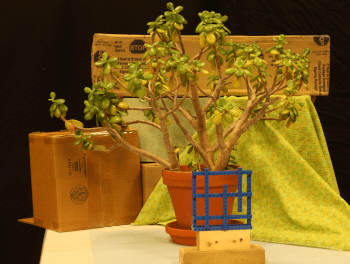
\includegraphics[width=3.6cm]{Figs/Introducao/exemplo_left.png}}}&
        \bmvaHangBox{\fbox{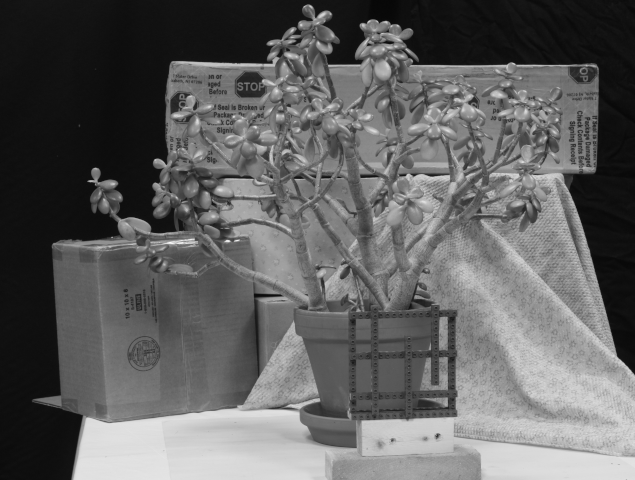
\includegraphics[width=3.6cm]{Figs/Metodologia/esq_480x635.png}}}&
        \bmvaHangBox{\fbox{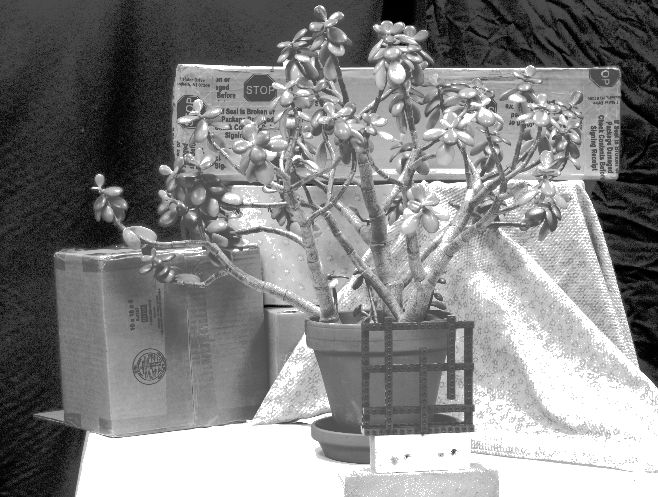
\includegraphics[width=3.6cm]{Figs/Metodologia/gray_left.png}}}\\
        (a)&(b)&(c)
    \end{tabular}
    \caption{Evolução do pré-processamento das imagens base, onde esta (a) é convertida para escala de cinza (b) e é ajustada (c).}
    \label{fig:met_pre_process}
\end{figure}

Com o caráter exploratório como principal objetivo, cinco algoritmos foram implementados:

\begin{enumerate}
    \item \textbf{OpenCV (OCV)}: método do algoritmo SBGM (\emph{Semi-Global Block Matching}) implementados pela biblioteca, gerando dois mapas de disparidades tendo ambas as imagens como base e pós-processando-os por intermédio da filtragem WLS (\emph{Weighted Least Squares}). Para tanto, uma exploração sobre a parametrização também foi realizada:~\emph{uniquenessRatio} (porcentagem de vantagem entre as duas melhores correspondências para sua confirmação),~\emph{speckleWindowSize} (tamanho máximo das regiões de disparidade suavizadas),~\emph{speckleRange} (variação máxima entre os componentes conectados),~\emph{wls\_lambda} (quantidade de regularização durante o filtro) e~\emph{wls\_sigma\_color} (sensibilidade às bordas durante a filtragmem);
    \item \textbf{Busca linear (BL)}: em cada linha retificada, considera-se como referência $\mathbf{R}$ (imagem da esquerda) um vetor de tamanho máximo $N$ e como janela de busca (imagem da direita) de tamanho máximo $M$. Com isso desliza-se uma janela do tamanho da referência obtida e a diferença entre janela deslizante $\mathbf{W}$ e a referência é computada, seguida pela busca da janela de menor diferença. A janela encontrada é validada considerando uma variação $|V|/\text{\emph{pixel}}$;
    \item \textbf{Correlação cruzada (CC)}: semelhante à~\emph{Busca linear} até o cálculo da diferença, visto que é computado ``o ângulo'' entre a janela deslizante e a referência: $(\mathbf{R} \cdot \mathbf{W})/(|\mathbf{R}| \cdot |\mathbf{W}|)$. A janela encontrada é validada considerando uma variação menor ou igual a $30º$ ($0,15$);
    \item \textbf{Janela deslizante (JD)}: semelhante à~\emph{Busca linear}, considera uma vizinhança 2D quadrada de tamanho fixo;
    \item \textbf{Janela deslizante adaptativa (JDA)}: semelhante à~\emph{Janela deslizante}, considera uma vizinhança 2D de tamanho variável controlada pela janela de busca.
\end{enumerate}

Ainda sob esta perspectiva, foram explorados diversos tamanhos ímpares para os blocos de verificação com $N \in [3, 17]$. Além disso, tanto os mapas de disparidade e de profundidade foram normalizados para comparação também.